% Informe técnico — Siniestros viales en Envigado
% Compilar con: latexmk -pdf informe_siniestros_viales_envigado.tex
\documentclass[11pt]{article}
\usepackage[T1]{fontenc}
\usepackage[margin=2.5cm]{geometry}
\setlength{\emergencystretch}{2em}
\setlength{\intextsep}{8pt plus 2pt minus 2pt}
\setlength{\abovecaptionskip}{6pt}
\setlength{\belowcaptionskip}{4pt}
\usepackage[spanish,es-tabla]{babel}
\usepackage{booktabs}
\usepackage{graphicx}
\usepackage{float}
\usepackage[font=small,labelfont=bf]{caption}
\usepackage{xcolor}
\usepackage{microtype}
\usepackage[colorlinks=true,linkcolor=blue!50!black,urlcolor=blue!50!black]{hyperref}

\hypersetup{pdftitle={Preparación de datos y clasificación de la gravedad de siniestros viales en Envigado}}

\newcommand{\vartxt}[1]{\texttt{#1}}

\title{Preparación de datos y clasificación de la gravedad de\\ siniestros viales en el municipio de Envigado, Colombia}
\author{Samuel Betancur \\ Fernando González \\ Juanita Correa}
\date{Octubre de 2026}

\begin{document}
\maketitle

\begin{abstract}
\noindent
A partir de 89.826 registros de accidentalidad vial del municipio de Envigado (2010--2022) publicados en el portal de Datos Abiertos de Colombia, se consolidaron 43.759 siniestros únicos y se ejecutó un pipeline completo de preparación de datos: reconciliación de formatos, eliminación de variables irrelevantes y redundantes, imputación de nulos, balanceo de clases y transformaciones. Con 8 variables predictoras se abordó la clasificación binaria de la gravedad del accidente (\vartxt{SOLO DAÑOS} frente a \vartxt{HERIDOS}), entrenando seis modelos de clasificación con búsqueda de hiperparámetros y validación cruzada de 10 folds. Aunque KNN obtuvo el mayor f1 en la comparación (0,80), se seleccionó \textbf{Random Forest} como modelo final por su mejor equilibrio entre desempeño y generalización: su f1 con validación en datos reales y balanceo dentro de cada fold es de 0,72, frente a los 0,67 de KNN, que además presentaba la mayor brecha de sobreajuste. El modelo se desplegó finalmente como aplicación web interactiva con Streamlit.
\end{abstract}

\section{Objetivo}

El presente informe documenta el proceso de preparación de datos y modelado de la accidentalidad vial del municipio de Envigado (Antioquia, Colombia), desarrollado en el notebook adjunto con Python (pandas, scikit-learn, imbalanced-learn, XGBoost y ydata-profiling).

El objetivo analítico es predecir la \textbf{variable objetivo} \vartxt{GRAVEDAD} como un problema de \textbf{clasificación binaria}: \vartxt{SOLO DAÑOS} frente a \vartxt{HERIDOS}. La clase \vartxt{MUERTOS}, con apenas el 0,3\,\% de los registros, se descarta por insuficiencia estadística (sección~\ref{sec:balanceo}). El trabajo cubre once fases: integración de los datos, eliminación de variables irrelevantes y redundantes, descripción estadística, limpieza de atípicos y de nulos, análisis de correlaciones, balanceo, transformaciones, persistencia de los datos preparados y, finalmente, el entrenamiento de seis modelos de clasificación con hiperparametrización (\vartxt{GridSearchCV} + validación cruzada).

\section{Descripción del conjunto de datos}

\textbf{Fuente.} Portal de Datos Abiertos de Colombia, conjunto ``Accidentalidad Municipio de Envigado'' (archivo CSV con corte al 29 de septiembre de 2026).

\textbf{Dimensionalidad y periodo.} El archivo crudo contiene \textbf{89.826 filas por 17 columnas}. No existe una correspondencia fila--accidente: cada siniestro aparece repetido una vez por cada vehículo o persona involucrada (un mismo \vartxt{RADICADO} llega a repetirse hasta 24 veces). Tras consolidar por \vartxt{RADICADO} quedan \textbf{43.759 siniestros únicos} (46.067 filas eran duplicados del mismo hecho), ocurridos entre el 1 de enero de 2010 y el 22 de junio de 2022.

\textbf{Calidad de datos.} El diagnóstico inicial evidenció:
\begin{itemize}\setlength\itemsep{0.1em}
  \item \emph{Unicidad} baja en el archivo crudo: 51\,\% de las filas correspondían a siniestros ya registrados; resuelta con la consolidación por \vartxt{RADICADO}.
  \item \emph{Conformidad} baja en \vartxt{FECHA} y \vartxt{HORA}: dos formatos distintos conviven en la misma columna, señal de que el dataset proviene de dos exportaciones o sistemas de captura concatenados.
  \item \emph{Completitud} crítica en seis columnas (entre 74\,\% y 99,9\,\% de nulos) y buena en las restantes (nulos reales $<0{,}01$\,\% una vez descartadas las columnas casi vacías).
  \item \emph{Consistencia}: valores tipo \vartxt{NO REPORTADA}/\vartxt{NO REPORTA} operan como nulos disfrazados dentro de categorías válidas.
  \item \emph{Exactitud} aceptable: no se detectaron valores fuera de rango en las variables numéricas codificadas.
  \item \emph{Actualidad} no verificable sin metadatos del proceso de captura.
\end{itemize}

\section{Descripción de las variables}

La Tabla~\ref{tab:variables} resume las 17 variables originales. Seis de ellas no tienen información aprovechable como predictoras por su altísimo porcentaje de nulos; las demás se usan a lo largo del pipeline.

\begin{table}[H]
\centering\small
\caption{Variables originales del conjunto de datos (porcentaje de nulos tras la consolidación por \vartxt{RADICADO}).}
\label{tab:variables}
\begin{tabular}{p{3.3cm} p{2.2cm} p{6.6cm} r}
\toprule
\textbf{Variable} & \textbf{Tipo} & \textbf{Descripción} & \textbf{\% nulos} \\
\midrule
\vartxt{RADICADO} & Identificador & Número único del siniestro & 0 \\
\vartxt{FECHA} & Fecha & Fecha del accidente (dos formatos mezclados) & 0 \\
\vartxt{HORA} & Hora & Hora del accidente (texto AM/PM y pseudo-fecha de Excel) & 0 \\
\vartxt{DÍA DE LA SEMANA} & Categórica & Día de ocurrencia & 0 \\
\vartxt{CLASE DE VEHICULO} & Categórica & Clase del vehículo involucrado & 99,55 \\
\vartxt{TIPO DE SERVICIO} & Categórica & Servicio del vehículo & 99,55 \\
\vartxt{TIPO DE VICTIMA} & Categórica & Rol de la víctima & 99,90 \\
\vartxt{SEXO} & Categórica & Sexo de la víctima & 99,90 \\
\vartxt{ESTADO DE BEODEZ} & Binaria & Estado de embriaguez (0/1) & 0 \\
\vartxt{RESULTADO DE BEODEZ} & Ordinal & Nivel de embriaguez (0--3) & 0 \\
\vartxt{GRAVEDAD} & Categórica & \textbf{Variable objetivo}: \vartxt{SOLO DAÑOS}, \vartxt{HERIDOS}, \vartxt{MUERTOS} & 0 \\
\vartxt{CLASE DE ACCIDENTE} & Categórica & Choque, atropello, caída, etc. & 0 \\
\vartxt{CAUSA} & Categórica & Causa registrada (405 categorías) & 0 \\
\vartxt{DIRECCIÓN} & Texto libre & Dirección del hecho & 98,29 \\
\vartxt{BARRIO} & Categórica & Barrio de ocurrencia (49 categorías) & 0 \\
\vartxt{AREA} & Categórica & Zona urbana o rural & 0 \\
\vartxt{Coordenadas} & Texto libre & Punto geográfico (WKT) & 74,14 \\
\bottomrule
\end{tabular}
\end{table}

\textbf{Variable objetivo.} \vartxt{GRAVEDAD} está fuertemente desbalanceada: 79,5\,\% \vartxt{SOLO DAÑOS}, 20,2\,\% \vartxt{HERIDOS} y 0,3\,\% \vartxt{MUERTOS} (Figura~\ref{fig:hora}, derecha).

\begin{figure}[H]
\centering
\begin{minipage}{0.48\textwidth}
\centering
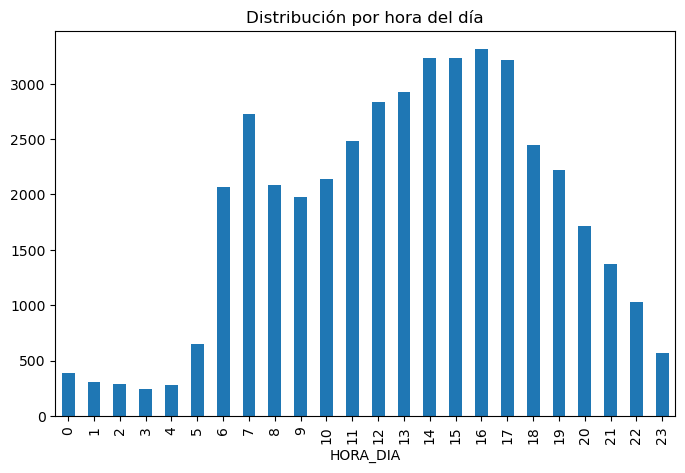
\includegraphics[width=0.95\textwidth]{figures/hora_dia_distribucion}
\end{minipage}\hfill
\begin{minipage}{0.48\textwidth}
\centering
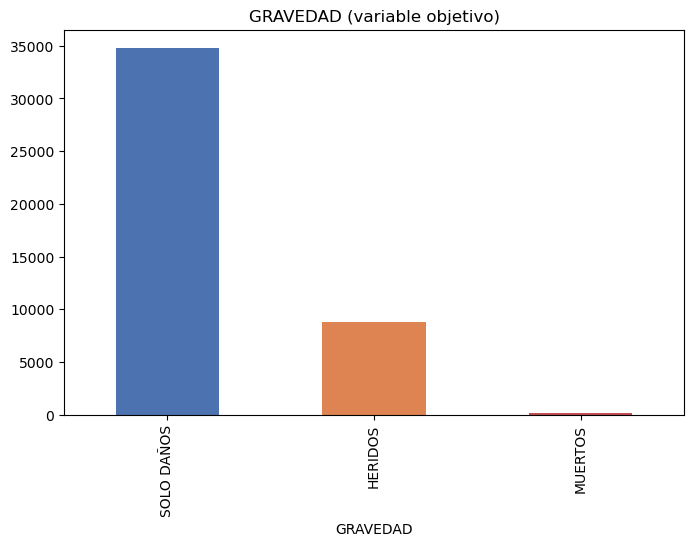
\includegraphics[width=0.95\textwidth]{figures/gravedad_antes_balanceo}
\end{minipage}
\caption{Izquierda: siniestros por hora del día (0--23 h). Derecha: distribución de la variable objetivo \vartxt{GRAVEDAD} antes del balanceo.}
\label{fig:hora}
\end{figure}

\textbf{Variables numéricas.} La hora del día (extraída de \vartxt{HORA}) tiene media 13,2 h, mediana 14 h y rango 0--23; el 50\,\% central de los accidentes ocurre entre las 9 y las 17 h (Figura~\ref{fig:hora}, izquierda), con una ligera concentración en la tarde. \vartxt{RESULTADO DE BEODEZ} es prácticamente constante en 0 (media 0,007; máximo 3): la inmensa mayoría de los conductores involucrados no presentaba embriaguez. Las variables categóricas se caracterizaron con diagramas de barras y un informe de perfilado automatizado (\vartxt{ydata-profiling}) exportado como HTML.

\section{Transformaciones y limpieza de datos}
\label{sec:limpieza}

\subsection{Integración y consolidación}

La fuente única no estaba integrada de forma homogénea, por lo que se resolvieron dos problemas:
\begin{enumerate}\setlength\itemsep{0.1em}
  \item \textbf{Un accidente $=$ varias filas.} Se consolidó por \vartxt{RADICADO} conservando la versión más reciente de cada siniestro (\vartxt{drop\_duplicates(keep='last')}), pasando de 89.826 filas a 43.759 siniestros únicos.
  \item \textbf{Formatos mixtos en fecha y hora.} \vartxt{FECHA} mezclaba texto \vartxt{DD/MM/AAAA} con formato ISO; se parseó con \vartxt{format='mixed'} y \vartxt{dayfirst=True}, y se descompuso en \vartxt{AÑO} y \vartxt{MES}. \vartxt{HORA} mezclaba texto en español (``10:30:00 p.\,m.'') con una pseudo-fecha de Excel (\vartxt{1899-12-31T14:30:00.000}, fecha ``cero'' al exportar solo la hora); una función dedicada reconoce ambos patrones y produce \vartxt{HORA\_DIA} (0--23) \emph{sin ningún fallo de interpretación}.
\end{enumerate}

\subsection{Eliminación de variables irrelevantes y redundantes}

Se eliminaron 7 variables \textbf{irrelevantes} (identificador o columnas sin información: \vartxt{RADICADO}, \vartxt{DIRECCIÓN}, \vartxt{Coordenadas} y las cuatro con más del 99\,\% de nulos) y 2 \textbf{redundantes} (\vartxt{FECHA} y \vartxt{HORA}, ya descompuestas en \vartxt{AÑO}, \vartxt{MES} y \vartxt{HORA\_DIA}).

Además se redujo la \textbf{cardinalidad} de las dos variables con demasiadas categorías: \vartxt{CAUSA} (405 categorías) se agrupó en las 15 causas más frecuentes (que explican el 88,6\,\% de los registros) más una categoría \vartxt{OTRA}; \vartxt{BARRIO} (49 categorías) en los 15 barrios más frecuentes (78,1\,\%) más \vartxt{OTRO}. Con ello se evita que el paso a variables dummy genere cientos de columnas casi vacías. El dataset quedó con 10 variables, todas con información útil.

\subsection{Limpieza de datos atípicos (errores de captura)}

Se verificó que las variables numéricas estuvieran dentro de su rango válido: \vartxt{ESTADO DE BEODEZ} $\in \{0,1\}$, \vartxt{RESULTADO DE BEODEZ} $\in \{0,1,2,3\}$, \vartxt{HORA\_DIA} $\in [0,23]$, \vartxt{AÑO} $\in [2010,2022]$; no se hallaron errores de rango. Los únicos errores detectados fueron 5 registros (0,011\,\%) con el valor \vartxt{NO REPORTADA}/\vartxt{NO REPORTA} en \vartxt{CLASE DE ACCIDENTE} (1) y \vartxt{AREA} (4): datos faltantes disfrazados de categoría, que se convirtieron a nulos explícitos.

\subsection{Imputación de nulos}

Ningún registro acumulaba múltiples nulos y las columnas con nulos masivos ya se habían eliminado, así que las dos columnas afectadas se imputaron por la \textbf{moda} con \vartxt{SimpleImputer}: \vartxt{CHOQUE} para clase de accidente, \vartxt{URBANA} para área (y de forma preventiva \vartxt{Otra-Conductor} y \vartxt{LAS VEGAS} para causa y barrio agrupados). Tras la imputación el dataset tiene \textbf{0 nulos}.

\subsection{Correlaciones: redundancias}

Codificando las categóricas como dummies (solo para el análisis) y aplicando el umbral $|r|>0{,}8$ se identificaron tres pares (Figura~\ref{fig:corr}):
\begin{itemize}\setlength\itemsep{0.1em}
  \item \vartxt{RESULTADO DE BEODEZ} vs.\ \vartxt{ESTADO DE BEODEZ} ($r=0{,}899$): redundancia real, pues el resultado ya contiene al estado como caso particular. Se eliminó \vartxt{ESTADO DE BEODEZ}, conservando la variable más informativa.
  \item \vartxt{AREA\_URBANA} vs.\ \vartxt{BARRIO\_VEREDA PALMAS} ($r=-0{,}871$): coincidencia esperada por definición geográfica (una vereda es zona rural por definición), no una redundancia de \vartxt{AREA}; no se tomó acción.
  \item \vartxt{GRAVEDAD\_HERIDOS} vs.\ \vartxt{GRAVEDAD\_SOLO DAÑOS} ($r=-0{,}990$): complementariedad matemática entre dummies del propio objetivo; no se tomó acción.
\end{itemize}

\begin{figure}[H]
\centering
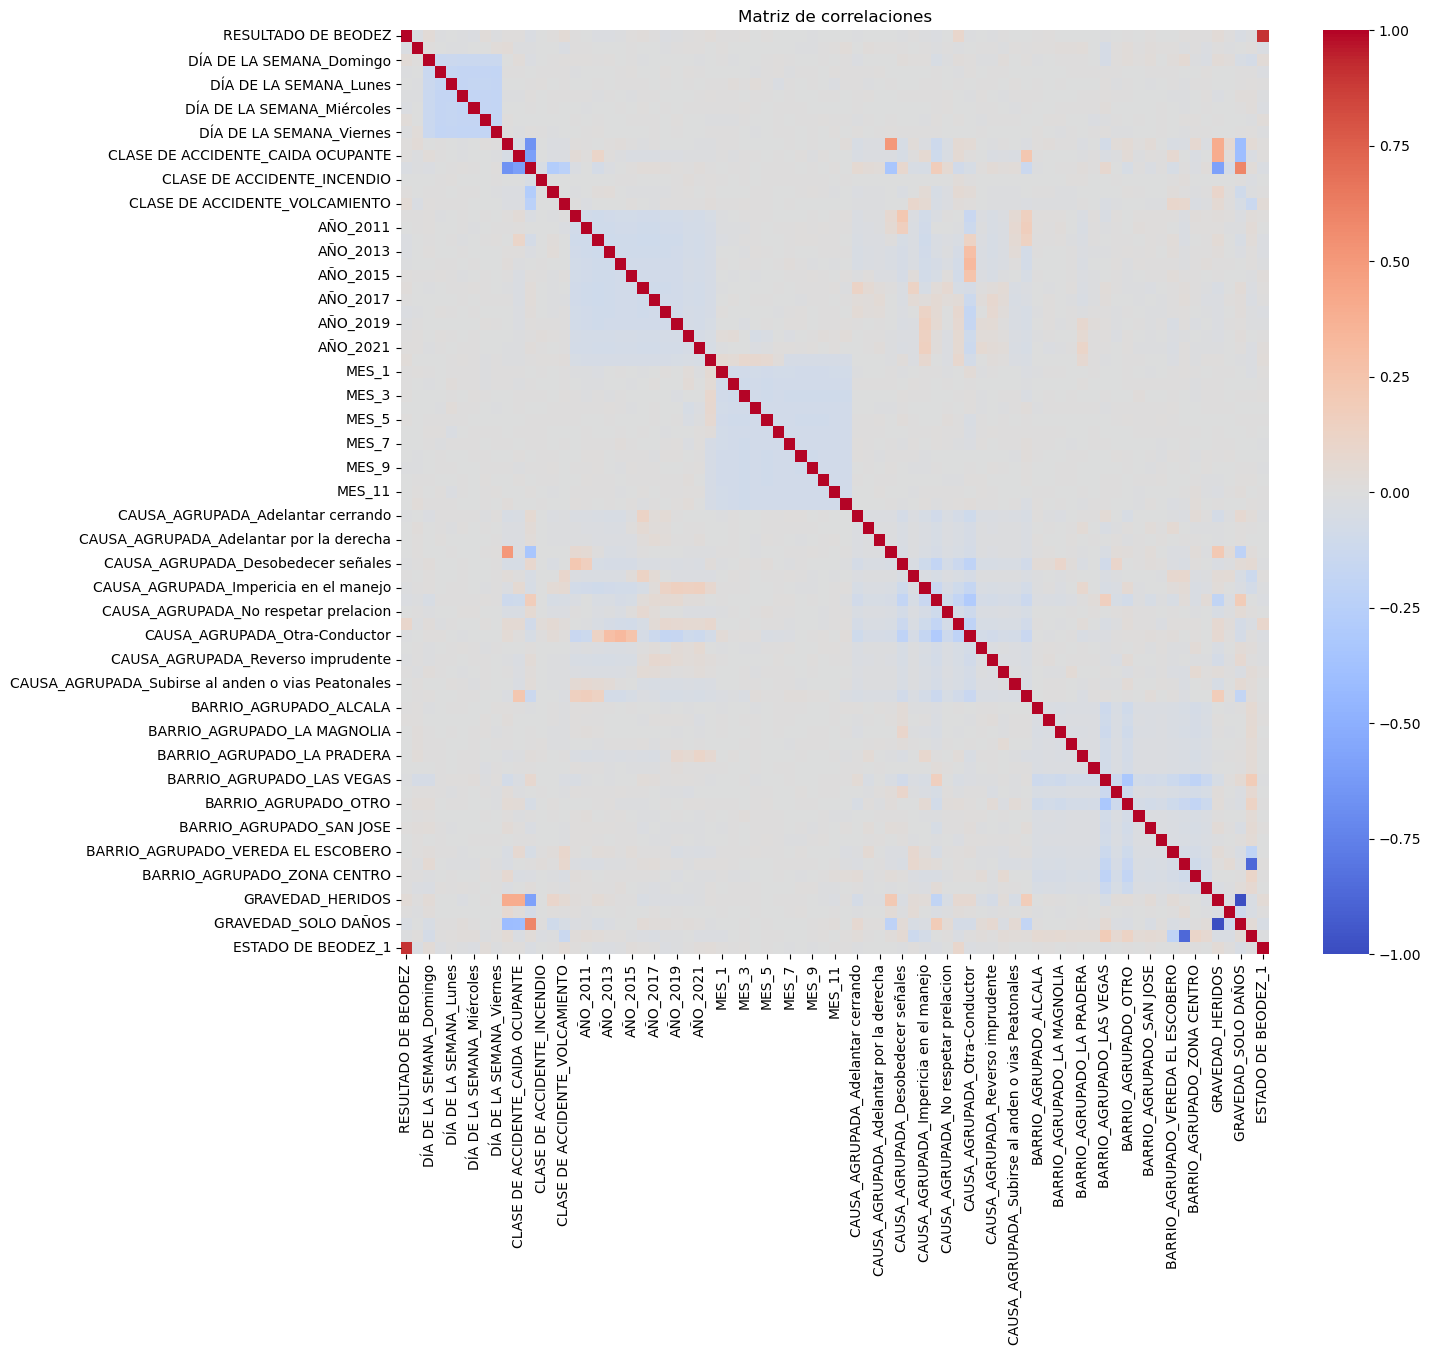
\includegraphics[width=0.68\textwidth]{figures/matriz_correlaciones}
\caption{Matriz de correlaciones del dataset codificado (variables dummy).}
\label{fig:corr}
\end{figure}

\subsection{Correlaciones: irrelevancia frente al objetivo}

Se calculó la correlación máxima absoluta de cada variable (agrupando sus dummies) frente a las dummies del objetivo (Tabla~\ref{tab:corr}). \vartxt{CLASE DE ACCIDENTE} (0,59) y \vartxt{CAUSA\_AGRUPADA} (0,22) son las variables con mayor señal. De las de señal mínima, solo se eliminó \vartxt{AÑO}: además de su correlación de 0,043, incluir el año exacto arriesga sobreajustar el modelo a los años observados y perjudicar la generalización a años futuros. Se conservaron \vartxt{HORA\_DIA}, \vartxt{DÍA DE LA SEMANA} y \vartxt{MES} pese a su baja correlación lineal, porque son variables \emph{cíclicas} (la hora 23 está ``cerca'' de la 0) y el coeficiente de Pearson subestima ese tipo de relaciones no monótonas.

\begin{table}[H]
\centering\small
\caption{Correlación máxima absoluta de cada variable frente al objetivo \vartxt{GRAVEDAD}.}
\label{tab:corr}
\begin{tabular}{lr}
\toprule
\textbf{Variable} & \textbf{Máx.\ $|r|$} \\
\midrule
\vartxt{CLASE DE ACCIDENTE} & 0,590 \\
\vartxt{CAUSA\_AGRUPADA} & 0,217 \\
\vartxt{BARRIO\_AGRUPADO} & 0,050 \\
\vartxt{ESTADO DE BEODEZ}$^{\ast}$ & 0,045 \\
\vartxt{AÑO} (eliminada) & 0,043 \\
\vartxt{DÍA DE LA SEMANA} & 0,039 \\
\vartxt{AREA} & 0,038 \\
\vartxt{RESULTADO DE BEODEZ} & 0,035 \\
\vartxt{MES} & 0,021 \\
\vartxt{HORA\_DIA} & 0,011 \\
\bottomrule
\multicolumn{2}{l}{\footnotesize $^{\ast}$Ya eliminada por redundancia (sección 4.5).}
\end{tabular}
\end{table}

Tras estas depuraciones quedan \textbf{8 variables predictoras finales}: \vartxt{DÍA DE LA SEMANA}, \vartxt{RESULTADO DE BEODEZ}, \vartxt{CLASE DE ACCIDENTE}, \vartxt{AREA}, \vartxt{MES}, \vartxt{HORA\_DIA}, \vartxt{CAUSA\_AGRUPADA} y \vartxt{BARRIO\_AGRUPADO}.

\subsection{Balanceo de la variable objetivo}
\label{sec:balanceo}

Un modelo entrenado con la distribución original (79,5/20,2/0,3) ignoraría las clases minoritarias. Las decisiones tomadas fueron:
\begin{enumerate}\setlength\itemsep{0.1em}
  \item \textbf{Eliminar la clase \vartxt{MUERTOS}} (0,3\,\%): no hay casos suficientes para aprender un patrón confiable y sobremuestrearla implicaría inventar casi todos sus registros. El problema pasa a ser binario: 43.616 siniestros (34.794 \vartxt{SOLO DAÑOS}, 8.822 \vartxt{HERIDOS}).
  \item \textbf{Submuestrear \vartxt{SOLO DAÑOS}} al 75\,\% de su tamaño (\vartxt{RandomUnderSampler}): 26.095 registros.
  \item \textbf{Sobremuestrear \vartxt{HERIDOS}} con \textbf{SMOTENC} (variante de SMOTE que soporta variables categóricas y numéricas mezcladas) hasta 13.047 registros.
\end{enumerate}
El resultado es un dataset de \textbf{39.142 registros} con proporción deliberada de \textbf{2:1} (Figura~\ref{fig:bal}): no se buscó el balance perfecto 50/50 para no introducir demasiados datos sintéticos ni descartar demasiados registros reales. Las filas se mezclaron para evitar que la validación cruzada concentre los registros sintéticos en los últimos folds, y se conservó una copia de los datos reales sin balancear (\vartxt{X\_real}/\vartxt{Y\_real}) para la verificación final de la sección~\ref{sec:resultados}.

\begin{figure}[H]
\centering
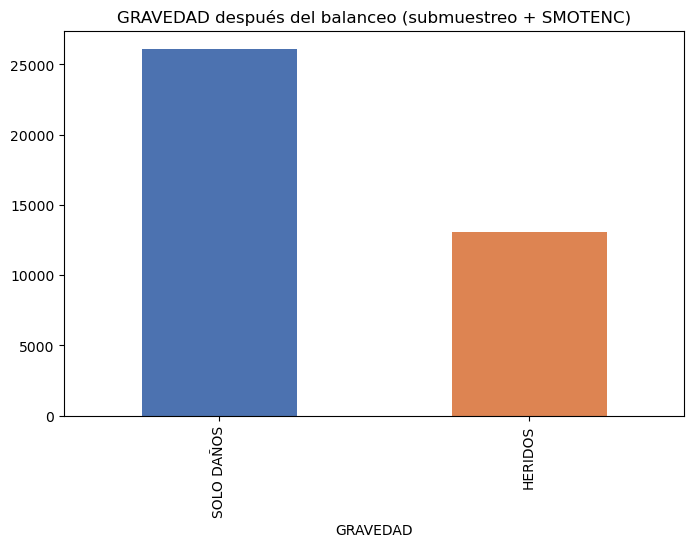
\includegraphics[width=0.42\textwidth]{figures/gravedad_despues_balanceo}
\caption{\vartxt{GRAVEDAD} después del balanceo: submuestreo de \vartxt{SOLO DAÑOS} al 75\,\% y sobremuestreo SMOTENC de \vartxt{HERIDOS} hasta la proporción 2:1.}
\label{fig:bal}
\end{figure}

\subsection{Transformaciones finales y persistencia}

Dependiendo del requisito del método de aprendizaje se prepararon \textbf{dos versiones} del dataset balanceado:
\begin{itemize}\setlength\itemsep{0.1em}
  \item \textbf{Versión categórica} (\vartxt{datos\_categoricos\_discretizados.xlsx}, $39142\times9$): discretización de \vartxt{HORA\_DIA} en franjas horarias --- \vartxt{Madrugada} (0--5), \vartxt{Mañana} (6--11), \vartxt{Tarde} (12--17), \vartxt{Noche} (18--23), Figura~\ref{fig:disc} --- y de \vartxt{RESULTADO DE BEODEZ} en \vartxt{Negativo}/\vartxt{Positivo}. Pensada para métodos categóricos (árboles, Bayes).
  \item \textbf{Versión numérica} (\vartxt{datos\_numericos\_}\allowbreak\vartxt{normalizados.xlsx}, $39142\times61$): normalización \vartxt{MinMax} de las numéricas al rango $[0,1]$, variables dummy para las categóricas (60 columnas predictoras) y \vartxt{LabelEncoder} para el objetivo (\vartxt{HERIDOS}$=0$, \vartxt{SOLO DAÑOS}$=1$). Es la versión empleada en el entrenamiento para que los seis modelos compitan sobre las mismas variables.
\end{itemize}

\begin{figure}[H]
\centering
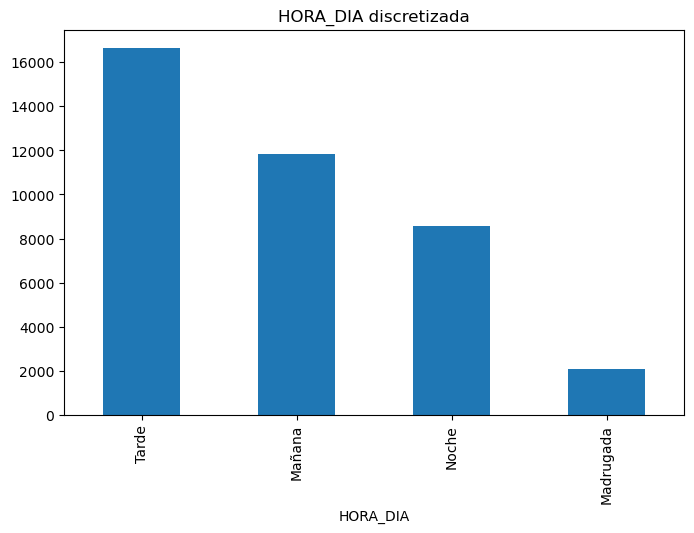
\includegraphics[width=0.42\textwidth]{figures/hora_dia_discretizada}
\caption{Discretización de \vartxt{HORA\_DIA} en franjas horarias (versión categórica del dataset).}
\label{fig:disc}
\end{figure}

\section{Entrenamiento de los modelos}
\label{sec:modelos}

Sobre la versión numérica del dataset (39.142 registros, 60 predictoras, objetivo binario) se entrenaron \textbf{seis modelos}: árbol de decisión, Random Forest, XGBoost, KNN, SVM y red neuronal (MLP). En lugar de dividir en entrenamiento/prueba (70/30), cada modelo se ajustó con \vartxt{GridSearchCV} usando \textbf{validación cruzada de 10 folds} y \textbf{f1 macro} como medida (adecuada para problemas con clases desbalanceadas, pues promedia el f1 de cada clase). El f1 promedio en los folds de entrenamiento (Train CV) frente al de validación (Test CV) permite revisar el sobreajuste. La Tabla~\ref{tab:grid} resume los espacios de hiperparámetros y la mejor configuración hallada por cada búsqueda.

\begin{table}[H]
\centering\small
\caption{Espacios de hiperparámetros evaluados y mejor configuración por modelo (\vartxt{GridSearchCV}, 10 folds, f1 macro).}
\label{tab:grid}
\begin{tabular}{p{2.6cm} p{7.2cm} p{4.6cm}}
\toprule
\textbf{Modelo} & \textbf{Hiperparámetros evaluados} & \textbf{Mejor configuración} \\
\midrule
Árbol de decisión & criterion: gini/entropy; min\_samples\_leaf: 2/10/50/100; max\_depth: None/10/20/50 & entropy, sin límite de profundidad, hojas de 10 registros \\
Random Forest & n\_estimators: 50/100/200; criterion: gini/entropy; max\_depth: None/10/20; min\_samples\_leaf: 2/10; max\_features: sqrt & 100 árboles, gini, sin límite de profundidad, hojas de 2 \\
XGBoost & n\_estimators: 100/200; max\_depth: 3/6/9; learning\_rate: 0{,}05/0{,}1/0{,}3; subsample: 0{,}8/1{,}0 & 200 árboles, profundidad 9, tasa 0{,}3, subsample 0{,}8 \\
KNN & n\_neighbors: 5/15/27; weights: uniform/distance & 27 vecinos, peso por distancia \\
SVM & kernel: rbf; C: 1/10 & rbf, C $=10$ \\
Red neuronal (MLP) & hidden\_layer\_sizes: (15,)/(64,32); activation: relu/logistic; early\_stopping & relu, una capa oculta de 15 neuronas \\
\bottomrule
\end{tabular}
\end{table}

\section{Resultados de calidad de los modelos}
\label{sec:resultados}

\begin{table}[H]
\centering\small
\caption{f1 macro en validación cruzada (10 folds), ordenado por desempeño en Test CV.}
\label{tab:resultados}
\begin{tabular}{lccc}
\toprule
\textbf{Modelo} & \textbf{f1 Train CV} & \textbf{f1 Test CV} & \textbf{Brecha} \\
\midrule
KNN & 0,9607 & \textbf{0,8013} & 0,159 \\
Random Forest & 0,8551 & 0,7854 & 0,070 \\
XGBoost & 0,8982 & 0,7853 & 0,113 \\
SVM & 0,8070 & 0,7630 & 0,044 \\
Árbol de decisión & 0,8091 & 0,7599 & 0,049 \\
Red neuronal (MLP) & 0,7574 & 0,7565 & 0,001 \\
\bottomrule
\end{tabular}
\end{table}

\textbf{Comparación entre modelos.} La Tabla~\ref{tab:resultados} y la Figura~\ref{fig:modelos} muestran que el mejor modelo es \textbf{KNN} (27 vecinos, peso por distancia) con un f1 macro de 0,8013, seguido muy de cerca por Random Forest (0,7854) y XGBoost (0,7853). En cuanto al diagnóstico de ajuste:
\begin{itemize}\setlength\itemsep{0.1em}
  \item \textbf{Sobreajuste:} KNN presenta la mayor brecha (f1 de entrenamiento 0,96 contra 0,80 en validación). Es esperable: con \vartxt{weights='distance'} cada registro de entrenamiento se predice prácticamente a sí mismo. XGBoost también muestra una brecha notable (0,113), mientras que Random Forest la controla (0,070) gracias al promedio de árboles.
  \item \textbf{Subajuste relativo:} la red neuronal y la SVM tienen los f1 de entrenamiento más bajos y brechas mínimas (0,001 y 0,044): generalizan de forma estable, pero con las configuraciones probadas no logran capturar todo el patrón.
\end{itemize}

\begin{figure}[H]
\centering
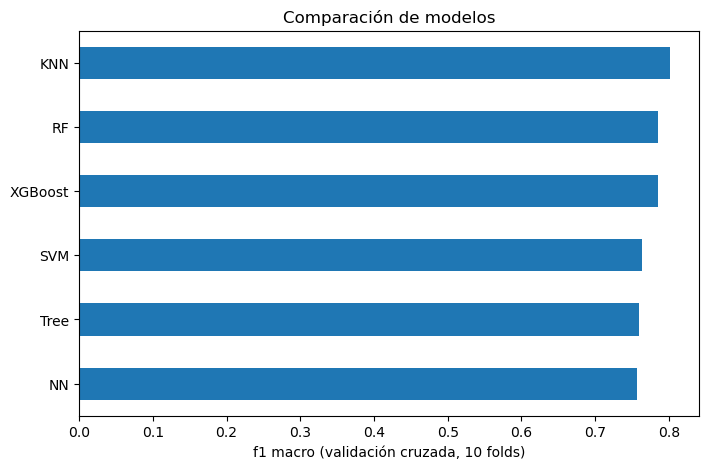
\includegraphics[width=0.46\textwidth]{figures/comparacion_modelos}
\caption{Comparación del f1 macro en validación cruzada de los seis modelos.}
\label{fig:modelos}
\end{figure}

\textbf{Verificación con datos reales.}\footnote{Los valores corresponden a la ejecución del notebook con \vartxt{random\_state=42}; pueden variar levemente entre ejecuciones o entornos.} El balanceo de la sección~\ref{sec:balanceo} se aplicó \emph{antes} de la validación cruzada, lo que hace que el f1 anterior pueda ser \textbf{optimista} por dos razones: (1) \emph{fuga de información}, pues los registros sintéticos de \vartxt{HERIDOS} se crean a partir de vecinos que luego caen en otros folds, y (2) \emph{validación sobre folds artificiales} con proporción 2:1 en lugar de la proporción real cercana a 80/20, en la que el f1 macro baja de forma natural porque la clase minoritaria es escasa.

Para obtener una estimación realista, el mejor modelo se reevaluó con los datos reales (\vartxt{X\_real}/\vartxt{Y\_real}) mediante un \vartxt{Pipeline} de imblearn que ejecuta el submuestreo, el sobremuestreo SMOTENC y la preparación de variables \textbf{solo dentro del fold de entrenamiento}, dejando cada fold de validación con accidentes reales en su proporción original. El resultado es:

\begin{center}
f1 con balanceo global: \textbf{0,8013} \quad$\rightarrow$\quad f1 con balanceo por fold: \textbf{0,6686 $\pm$ 0,0061} \quad(diferencia: 0,1327)
\end{center}

La caída combina ambos efectos. KNN es especialmente sensible a la fuga de SMOTENC: un registro sintético casi siempre tiene como vecino más cercano al registro real del que fue generado.

\textbf{Selección del modelo final.} Aunque KNN encabezó la comparación con validación cruzada, se seleccionó \textbf{Random Forest} como modelo final por ofrecer el mejor equilibrio entre desempeño y generalización: su f1 en validación (0,7854) es prácticamente igual al de KNN, pero su brecha de sobreajuste es menos de la mitad (0,070 frente a 0,159). Además, al ser un método basado en árboles, Random Forest es menos sensible a la fuga de información del sobremuestreo sintético: al repetir la verificación con datos reales y balanceo por fold (mismo protocolo que para KNN), su f1 realista es de \textbf{0,7159 $\pm$ 0,0074} ---una caída de apenas 0,070 desde el balanceo global, frente a los 0,1327 de KNN---, lo que lo convierte en el modelo con mejor desempeño esperado en producción. Las cifras de la Tabla~\ref{tab:resultados} sirven para \emph{comparar} modelos entre sí; el valor realista a reportar es el de la verificación por fold.

\section{Despliegue}
\label{sec:despliegue}

El modelo seleccionado (Random Forest) se puso en producción mediante una aplicación web interactiva desarrollada con \textbf{Streamlit} (\vartxt{app\_siniestros\_viales.py}), acompañada de un archivo \vartxt{requirements.txt} que fija las dependencias del despliegue (streamlit, pandas, scikit-learn, joblib, imbalanced-learn, xgboost).

\textbf{Artefacto del modelo.} El notebook serializa en \vartxt{modelo-siniestros.pkl} todo lo necesario para inferir: el modelo entrenado, el codificador de la variable objetivo, la lista de columnas predictoras en el orden del entrenamiento, el escalador \vartxt{MinMax} y las opciones de los menús desplegables. Como el modelo final es un método basado en árboles ---insensible a la escala de las variables numéricas---, se entrenó con \vartxt{HORA\_DIA} y \vartxt{RESULTADO DE BEODEZ} en su escala original; la aplicación replica exactamente esa codificación al construir la matriz de entrada, de modo que la inferencia reproduce fielmente el entrenamiento.

\textbf{Funcionamiento de la aplicación.} El usuario selecciona los ocho factores del siniestro (mes, hora del día en formato hh:00, día de la semana, área, barrio, clase de accidente, resultado de beodez y causa registrada). Al enviar el formulario, la aplicación activa las columnas dummy correspondientes, reconstruye las 60 columnas en el orden de entrenamiento y muestra la clasificación estimada (\vartxt{HERIDOS} o \vartxt{SOLO DAÑOS}), junto con los datos utilizados en la consulta (Figura~\ref{fig:ui}).

\begin{figure}[H]
\centering
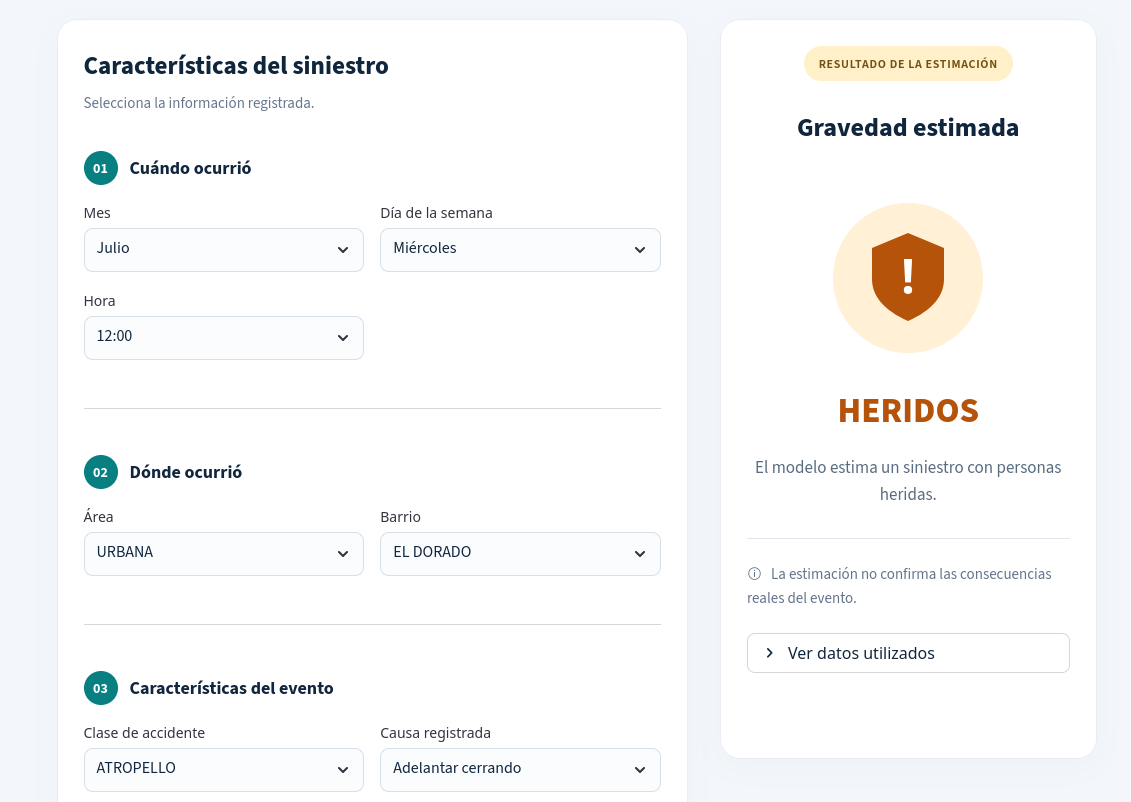
\includegraphics[width=0.68\textwidth]{figures/app-screenshot}
\caption{Interfaz de la aplicación Streamlit de estimación de gravedad de siniestros viales.}
\label{fig:ui}
\end{figure}

\section{Conclusiones}

\begin{itemize}\setlength\itemsep{0.15em}
  \item El pipeline de preparación transformó un archivo crudo de 89.826 filas $\times$ 17 columnas ---con siniestros duplicados, formatos mixtos de fecha/hora y columnas casi vacías--- en un conjunto de 43.759 siniestros únicos descrito por 8 variables predictoras limpias, sin nulos y con cardinalidad controlada, del que se derivaron dos versiones persistidas (categórica discretizada y numérica normalizada).
  \item La mayor señal predictiva la aportan \vartxt{CLASE DE ACCIDENTE} (máx.\ $|r|=0{,}59$) y \vartxt{CAUSA\_AGRUPADA} (0,22); el resto de variables tiene correlación lineal mínima con la gravedad, aunque las cíclicas (hora, día de la semana, mes) se conservaron porque la correlación de Pearson subestima relaciones no monótonas.
  \item En la comparación con validación cruzada, KNN fue el mejor modelo (f1 macro 0,8013), seguido de Random Forest y XGBoost; los modelos más flexibles encabezan el ranking, pero también muestran mayor brecha de sobreajuste.
  \item La verificación con datos reales demostró que balancear antes de la validación cruzada infla la medida: el f1 realista de KNN es 0,6686 $\pm$ 0,0061 y el de Random Forest es 0,7159 $\pm$ 0,0074. El protocolo correcto ---balancear únicamente dentro del fold de entrenamiento--- es la cifra que debe reportarse.
  \item El balanceo por remuestreo no es la única alternativa: árbol, Random Forest, XGBoost y SVM pueden manejar el desbalance con pesos de clase (\vartxt{class\_weight='balanced'} o \vartxt{scale\_pos\_weight}) entrenando con datos reales, mientras que KNN y la red neuronal sí requieren el remuestreo. Se usó el mismo balanceo para los seis modelos con el fin de compararlos en igualdad de condiciones.
  \item \textbf{Modelo final: Random Forest.} Aunque KNN obtuvo el mayor f1 en la comparación con validación cruzada (0,8013 frente a 0,7854), se seleccionó Random Forest por dos razones: (1) su brecha de sobreajuste es menos de la mitad de la de KNN (0,070 frente a 0,159), y (2) es menos sensible a la fuga de información del sobremuestreo, como confirmó la verificación con datos reales, donde supera a KNN (0,7159 frente a 0,6686). En consecuencia, Random Forest es el modelo con mejor desempeño esperado en producción.
  \item El modelo seleccionado se desplegó como aplicación web Streamlit que, a partir de los ocho factores del siniestro, reconstruye la matriz de entrada del modelo y devuelve la gravedad estimada; el artefacto serializado (\vartxt{modelo-siniestros.pkl}) incluye el modelo, el codificador, el escalador y las opciones de los desplegables, de modo que la inferencia es reproducible fuera del notebook.
\end{itemize}

\end{document}